\section{Opérateurs de flux}
L'avantage de la gestion de flux est de pouvoir gérer la dynamique des données via des opérateurs dédiés. Astral est construite sur la sémantique a deux concepts, il nous faut donc définir les opérateurs flux vers relation (fenêtres) et relation vers flux (streamers). Puis, nous définirons et explorerons des opérateurs spécifiques à la gestion de flux étant : la gestion des modifications des relations et des \textit{batchs}.
\subsection{Fenêtres}
L'opérateur de fenêtre est un des opérateurs les plus étudiés dans la littérature. Toutefois, son comportement est encore flou sur certains points. La formalisation de son fonctionnement permettra donc une meilleure compréhension.
\subsubsection{Association position-\textit{batch}}
Avant de définir formellement l'opération de fenêtrage, nous avons besoin d'un outil pour gérer l'association entre la position d'un n-uplet et de son \textit{batch}. La fonction $\tau_S$ définit cette association. 
\begin{defi}[Fonction position-\textit{batch}]\label{def:tau}
    Soit $S$ un flux,

    La fonction $\tau_S : \N\cup\{-1\}\to \TN$ est la fonction associant un entier à l'identifiant de \textit{batch} du seul n-uplet présent à cette position.

    Par convention, $\tau_S(-1)=(t_0,0)$.
\end{defi}

Par corollaire de l'hypothèse fondamentale~\ref{hyp:ordres}, la fonction $\tau_S$ est donc croissante non-stricte. Ainsi, il est possible de définir une pseudo inverse $\rtau_S$ capable de donner une position (la maximale en l'occurence) pour un \textit{batch} donné.
\begin{coro}[Fonction pseudo-inverse $\tau$]
    Soit $S$ un flux,

    La pseudo-inverse $\rtau_S:\TN\to \N\cup\{-1\}$ existe et correspond à la plus grande position du \textit{batch} donné en entrée. Si aucun \textit{batch} n'existe, le plus proche est utilisé. Formellement, $$\forall b \in \TN, \qquad \tau_S^{-1}(b) = \sum_{n=-1}^{+\infty} n \indic_{[\tau_S(n),\tau_S(n+1)[}(b)$$
\end{coro}

De par sa nature, la fonction $\tau$ et sa pseudo-inverse partagent des propriétés intéressantes que nous pourrons réutiliser lors de démonstrations formelles.
\begin{prop}[Propriétés de $\tau$]
    Soit $S$ un flux, alors les propriétés suivantes sont correctes :
    \begin{eqnarray*}
        t_0 & \leq & \tau_S(0) \\
        \tau_S(\tau_S^{-1}(b)) & \leq & b \\
        n & \leq & \tau_S^{-1}(\tau_S(n))
    \end{eqnarray*}

    De plus, si $\exists s \in S$, $\BS(s)=b$, alors $\tau_S(\tau_S^{-1}(b)) = b$.
\end{prop}
\subsubsection{Description de séquences de fenêtres}
Afin de se rapproche le plus possible d'un aspect déclaratif, nous souhaitons décorréler l'opérateur de fenêtre en deux objets mathématiques : la description et l'opérateur exécutable. Ce dernier prendra une description en argument pour pouvoir représenter la relation temporelle résultante. Le principe des descriptions de séquences de fenêtres est assez simples, il suffit de décrire deux bornes évoluant de manière discrête, et un taux d'évaluation de ces bornes.

\begin{defi}[Description de Séquence de Fenêtre (DSF)]
    Soient $\D$ et $\D'$ pouvant être $\T$ ou $\N$, une description de séquence de fenêtre (DSF) est un triplet $(\alpha,\beta,r)$ tel que :
\begin{itemize}
    \item $r \in \D$ est le taux d'évaluation des bornes de la fenêtre
    \item $\alpha$ et $\beta$ sont deux fonction de $\N\to D'$ représentant l'évolution des bornes.
\end{itemize}

$\alpha(j)$ et $\alpha(j)$ définissent les $j\eme$ valeures des bornes. La première étant donnée pour $j=0$. Ces fonctions se doivent de vérifier les propriétés suivantes (en considérant $\D=\D'=\T$) :
$$\forall j \in \N, \begin{cases} \alpha(j) \leq \beta(j) & \textrm{le début est avant la fin}\\ \alpha(j) \geq t_0 & \textrm{le début existe} \\ \beta(j) \leq jr + \beta(0) & \textrm{la fin est accessible} \end{cases}$$
    Les conditions pour les autres cas pour $\D$ et $\D'$ sont évidentes par application des fonctions $\tau_S$ et $\tau_S^{-1}$.
\end{defi}

\begin{example}
    Nous souhaitons relever tous les $100$ relevés de charge processeur, les $10$ derniers relevés. Dans ce cas, nous souhaitons obtenir une séquence de fenêtres positionnelles générées tous les $100$ n-uplets ($r=100\in \N$). Nous appliquons des bornes positionnelles donc $\alpha,\beta \in (\N\to\N)^2$. La première fenêtre couvrira du $91\eme$ n-uplet au $100\eme$. Ainsi : $\alpha(0) = 91$ et $\beta(0) = 100$. L'évolution des bornes étant linéaire, nous avons donc :
\begin{eqnarray*}
 \alpha(j) &=& 100j+91\\
 \beta(j) &=& 100j + 100\\
 r & = & 100
\end{eqnarray*}
\end{example}

La création de fenêtre nécessite l'association entre les n-uplets du flux et le numéro de fenêtre décrit dans la \textit{DSF}. Pour cela, nous utilisons une \textit{fonction d'attente} utilisant les identifiants de \textit{batch}. Cette fonction donne le rang de la dernière fenêtre au moment indiqué par le batch. Le terme \textit{attente} est lié au fait que l'évaluateur devra attendre avant le prochain changement de $\gamma$.
Nous retrouvons dans cette fonction le caractère \textit{bloquant} des fenêtres.
\begin{defi}[Fonction d'attente $\gamma$]
    Soit $S$ un flux, soit $(\alpha,\beta,r)$ une DSF,

    La fonction d'attente de la DSF est une fonction $\TN \to \N$ associant un identifiant de \textit{batch} à l'identifiant de la dernière fenêtre complétée.
\begin{itemize}
 \item  Si $r\in\T$, cette fonction est définie par $\gamma : (t,i) \mapsto \left\lfloor \frac{t-\beta(0)}{r} \right\rfloor$.
 \item  Si $r\in\N$, cette fonction est définie par $\gamma : (t,i) \mapsto \left\lfloor \frac{\rtau_S(t,i)-\beta(0)}{r} \right\rfloor$.
\end{itemize}
\end{defi}
\begin{example}
    En reprenant l'exemple précédent, après simplification nous obtenons : $$\gamma(b) = \left\lfloor \frac{\rtau_S(b)}{100}\right\rfloor-1.$$
    Si nous supposons que le flux produit un n-uplet par seconde (ainsi, $\rtau_S(t,i) = \lfloor t/1s \rfloor$) : alors $\gamma(1024s,0) = \left\lfloor \frac{1024}{100}\right\rfloor-1 = 9$. Nous avons donc bien la $10\eme$ fenêtre ($j=9$) comme la dernière fenêtre créée à ce moment.
\end{example}

\subsubsection{L'opérateur}
Il devient désormais possible de définir un opérateur permettant  de générer une relation temporelle à partir d'un flux donné. Cette relation temporelle gère ses changements d'état grâce à la fonction $\gamma$. De manière générale, une DSF peut être ramenée simplement à une expression plus générale $(\alpha,\beta,\gamma)$ ce que nous utiliserons pour la définition de séquence de fenêtres.
\begin{defi}[Opérateur de Séquence de Fenêtres]
	Soit $S$ un flux et $(\alpha, \beta, \gamma)$ une description de séquence,
	
	L'opérateur de séquence de fenêtres est défini par : $\forall b \in \TN$, 
	\begin{itemize}
		\item Si $\gamma(b) \geq 0$, 
		\begin{itemize}
			\item Si la description possède des bornes temporelles :
			$$S[\alpha,\beta,\gamma](b) = \left\{s\in S, \ (\alpha(\gamma(b)),0)\leq \BS(s) \leq (\beta(\gamma(b)),i)\right\}$$
			\item Si la description possède des bornes positions :
			$$E(b) = \left\{s\in S, \ \tau_S(\alpha(\gamma(b)))\leq \BS(s) \leq \tau_S(\beta(\gamma(b)))\right\}$$
			$$S[\alpha,\beta,\gamma](b) = \{s \in E(b) / (\#E(b) - \pos_{E(b)}(s)) \leq \beta(\gamma(b)) - \alpha(\gamma(b))$$
		\end{itemize}
		\item Si $\gamma(b) <0$ alors $S[\alpha,\beta,\gamma](b) = \emptyset$
	\end{itemize}
\end{defi}

Plusieurs remarques peuvent être formulées sur cette définition. Tout d'abord, les expressions sont différentes si les bornes sont positionnelles ou temporelles. Pour les fenêtres temporelles, l'opérateur inclue les n-uplets dont l'identifiant de \textit{batch} s'étend :
\begin{itemize}
	\item[\textbf{depuis}] le premier \textit{batch} de la fenêtre : $(\alpha(\gamma(t,i)),0)$, i.e. ceux dont le \textit{timestamp} est supérieur à la borne inférieur.
	\item[\textbf{jusqu'au}] dernier \textit{batch} de la fenêtre : $(\beta(\gamma(t,i)),i)$. Ce qui correspond au $i\eme$ \textit{batch} ayant le \textit{timestamp} inférieur ou égal à la borne.
\end{itemize}
Il est important de voir que $S[\alpha,\beta,\gamma]$ pourra changer à l'arrivée d'un nouveau \textit{batch}, même si le \textit{timestamp} ne change pas. Ne pas inclure ces modifications ferait perdre des données de dynamicités à la fenêtre. Nous retrouvons donc les problématiques explorées dans la section~\ref{sec:rw:sgfd:modeles}.

Pour les fenêtres positionnelles, la gestion est plus délicate. Si nous considérons que le flux réparti ses \textit{batchs} (donc un n-uplet par \textit{batch}), alors $E(b) = S[\alpha,\beta,\gamma](b)$. Mais dans le cadre général, $E(b)$ contient l'ensemble des n-uplets potentiels et la séquence $S[\alpha,\beta,\gamma](b)$ en est un sous-ensemble dont la taille est exactement celle décrite dans la DSF (sélections des n-uplets les plus récents). De plus, nous remarquons que $\gamma$ en positionnel est dirigé par $\rtau_S$ qui fournit la position maximale en cas d'égalité de \textit{batch}, ce qui nous garanti de couvrir l'ensemble des n-uplets concernés.

	
\begin{example}
	La figure~\ref{fig:contrib:astral:fenetres} montre l'évolution d'une séquence où la fenêtre glisse de $2$ secondes toutes les $2$ secondes ($r=2$) avec une taille constante de $3$ secondes. $t_0 = 0$ par simplicité ici. 
La première fenêtre possède les bornes $\alpha(0) = t_0+ 0s$ et $\beta(0) =t_0+3s$. Le glissement étant de $2s$ la description de fenêtre est donc $$\forall j \in \N, \begin{cases} \alpha(j)  & =\ j*2s+t_0 \\ \beta(j) & = \ j*2s+3s+t_0\end{cases}$$
La relation temporelle généré par cette DSF peut être noté $S[2js,2js+3s,2s]$.  Le calcul de son état à un instant est simple. Prenons le batch $(t_0+5.5s,0)$. La fenêtre a calculer est la fenêtre numérotée $\gamma(t_0+5.5s,0) = \left\lfloor \frac{t_0+5.5s-\beta(0)}{r}\right\rfloor = 1$. Ainsi : $S[2js,2js+3s,2s](t_0+5.5s,0) = F_1 = \{s_4,s_5,s_6,s_7,s_8\}$.
\end{example}
\begin{figure}[ht]
	\centering
	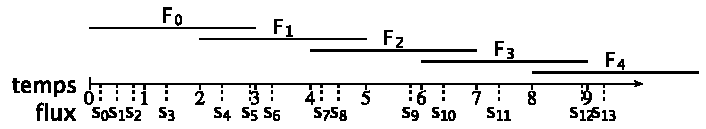
\includegraphics[width=0.7\textwidth]{contrib-astral-fenetres}
	\caption{Séquence de fenêtre de taille $3s$ glissante de $2s$}\label{fig:contrib:astral:fenetres}
\end{figure}

\begin{defi}[Exclusions de bornes de fenêtres]
    Soit $S$ un flux et $(\alpha,\beta,\gamma)$ une description de séquence de fenêtre,

    La notation $S]\alpha,\beta,\gamma]$, $S[\alpha,\beta,\gamma[$ et $S]\alpha,\beta,\gamma[$ désignent les définitions de l'opérateur classique de séquence de fenêtre permettant d'exclure respectivement les bornes inférieure, supérieure ou toutes.
\end{defi}

\begin{example}
    En reprenant une définition de fenêtre déjà abordée étant la fenêtre sur 5 secondes : $(j*5s+t_0,j*5s+5s+t_0,5s)$. Nous remarquons qu'entre la fenêtre 0 et 1, les n-uplets dont le \textit{timestamp} est égal à $t_0+5s$ seront dans ces deux fenêtres. Ainsi, l'opérateur $S]jr+t_0,jr+r+t_0,r]$ avec $r=5s$ permettra de retirer ce timestamp de cette fenêtre.
\end{example}


\subsubsection{Fenêtres partitionnées}
L'opérateur de fenêtres partitionnée est très utilisé pour appliquer la même séquences de fenêtres à des sous-flux. Les opérateurs partitionnés sont tous décrit de la même manière. Le principe, illustré dans la figure~\ref{fig:contrib:astral:partition} est de divisé le flux suivant un (ou des) attributs $A$ donné. Sur chacun de ces sous-flux est appliqué un opérateur quelconque. Par la suite, une union est appliquée.
\begin{figure}[ht]
	\centering
	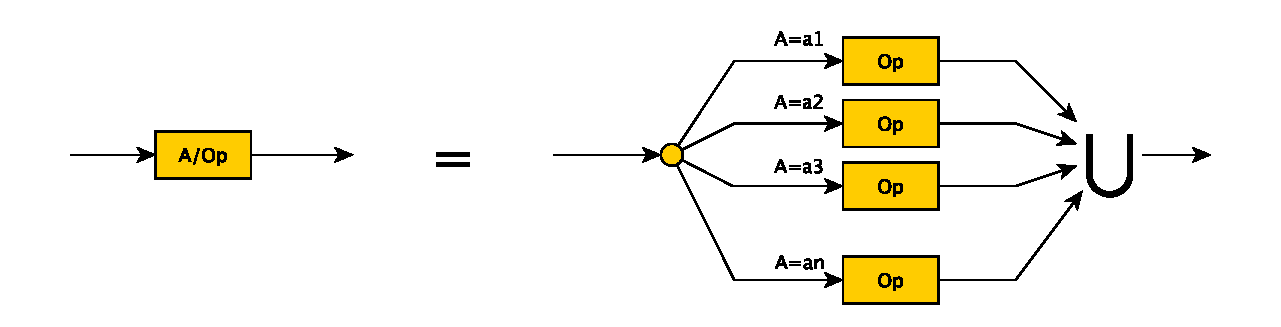
\includegraphics[width=0.9\textwidth]{contrib-astral-partition}
	\caption{Principe d'un opérateur partitionné}\label{fig:contrib:astral:partition}
\end{figure}
\begin{defi}[Séquence de fenêtre partitionnée]
	Soient $S$ un flux, $a_1,...,a_k$ un ensemble d'attributs du schéma de $S$, et $(\alpha,\beta,\gamma)$ une DSF,
	
	Soit $\cup^*$ l'union relationnelle conservatrice des identifiants physiques, 

	Alors la séquence de fenêtre $(\alpha,\beta,\gamma)$ partitionnée par $a_1,...,a_k$ est définie par :
	$$S[a_1...a_k/\alpha,\beta,\gamma] = \mathop{\bigcup\null^*}_{a\in Dom(a_1,...,a_k)} (\sigma_{(a_1,...,a_k)=a} S)[\alpha,\beta,\gamma]$$
\end{defi}

Nous remarquons que nous utilisons la définition conservatrice de l'union relationnelle présenté dans la section précédente, ainsi l'ordre naturel décrit dans le flux d'entrée pourra être retrouvé dans la relation de sortie.
\begin{example}
	L'exemple le plus courant étant la représentation de l'état actuel d'un système à partir d'un flux. Supposons un flux d'entrée $DeviceCPU(deviceId,cpu,\t)$, nous donnant les relevés de charge de processeur. Soit la description de fenêtre rapportant le dernier n-uplet d'un flux : $(1j,1j,1)$. Nous pouvons obtenir la relation temporelle représentant pour chaque dispositif $deviceId$, la dernière valeure connue de $cpu$ et son \textit{timestamp de mesure} $\tau$ : $$DeviceCPU[id/1j,1j,1]$$

	Cet exemple illustre comment nous pouvons passer d'un flux brut à une représentation (dynamique) d'un \textbf{contexte}.
\end{example}

Par la suite, nous utiliserons plusieurs notations simplifiés pour désigner des descriptions de fenêtres courantes décrites dans le tableau~\ref{tab:windows}.
\begin{table}[ht]
\centering
\begin{tabular}{c||p{0.4\textwidth}|p{0.4\textwidth}}
  & Définition & Équivalence \\ \bottomrule
 $[L]$ & $[j,j,1]$ &  \\ 
 & \multicolumn{2}{p{0.8\textwidth}}{La séquence de fenêtre où chaque fenêtre ne contient que le dernier n-uplet du flux. Cette séquence est égale à $[B]$ si le flux réparti ses n-uplets avec un n-uplet par \textit{batch}.} \\ \hline
 $[B]$ & $]\tau_S^{-1}(\tau_S(j)^-),j,1]$ & $\{s\in S, \BS(s) = \tau_S\circ\tau_S^{-1}(b)\}$ \\ 
 & \multicolumn{2}{p{0.8\textwidth}}{Séquence de fenêtre où chaque fenêtre contenient le dernier \textit{batch}.} \\\hline
 $[\infty]$ & $[0,j,1]$ & $\{s\in S, \BS(s) \leq b\}$ \\
 & \multicolumn{2}{p{0.8\textwidth}}{Séquence accumulative contenant tout le flux jusqu'au \textit{batch} courant.} \\\hline
 $[T\ r\ s]$ & $]\max(sj-r+t_0,t_0),sj+t_0,s]$ &  \\
 & \multicolumn{2}{p{0.8\textwidth}}{Fenêtre temporelle de taille $r$ se déplaçant toutes les $s$ unités de temps.} \\\hline
 $[P\ r\ s]$ & $]\max(sj-r,0),sj,r]$ &  \\
 & \multicolumn{2}{p{0.8\textwidth}}{Fenêtre positionnelle de taille $r$ n-uplets se déplaçant tous les $s$ n-uplets.} \\
 \toprule
\end{tabular}
\caption{Liste des fenêtres courantes} \label{tab:windows}
\end{table}

Il est important de noter que les équivalences citées sont toutefois non triviales, des démonstrations formelles sont fournies en annexes.

\subsection{Streamers}
La classe des \textit{streamers} est l'ensemble des opérateurs produisants un flux à partir d'une relation. Son utilisation est souvent appliquée après l'application d'une fenêtre pour permettre la recréation d'un flux après avoir travaillé dans le relationnel. Sa définition est découpée en deux parties, tout d'abord la définition de la réécriture de \textit{timestamp} permettant d'ajouter le \textit{timestamp} aux données produites, et ensuite la définition de l'opérateur en soit.
\subsubsection{Réécriture de \textit{timestamp}}
La réécriture de \textit{timestamp} est important pour modifier les n-uplets de $R$ avant leur mise sous forme de flux. Tout d'abord, il est nécessaire de correctement gérer les identifiants physiques. En effet, si un n-uplet est envoyé plusieures fois dans le flux résultant, il y aura un conflit si $\varphi$ n'est pas modifié. De plus, tout flux doit avoir un attribut $\t$ par définition. Cet attribut doit être créé ou remplacé pour assurer l'hypothèse de ordres. Le principe étant que si nous souhaitons envoyer le n-uplet $s\in R(b)$ dans le flux au \textit{batch} $(t_s,i_s)$, alors nous devons envoyer le n-uplet $\Psi_b(s,t_s)$.
\begin{defi}[Fonction de réécriture de \textit{timestamp}]
    Soit $R$ une relation de schéma $A$, $b$ un batch,

    Soit $\Phi_b^S$ une application $\I_{R} \to \I^S$ étant une fonction strictement croissante telle que : 
        $\forall b'\leq b, \ \forall i\in \I_R, \ \Phi_{b'}^S(i) \leq \Phi_b^S(i)$

    La fonction de réécriture de \textit{timestamp} appliquée à $R(b)$ est définie par : 
$$\forall s\in R(b), \ \forall t_s\in\T, \ \Psi_b(s,t_s) = \{(\t,t_s), (\varphi, \Phi_b^S(\varphi))\}\bigcup_{a\in A\backslash\{\varphi,\t\}}\{(a,s(a))\}$$
\end{defi}

Cette définition assure donc que les nouveaux n-uplets formant le flux vérifieront les propriétés suivantes : 
\begin{itemize}
 \item Ils ont pour \textit{timestamp} $t_s$ correspondant au moment où il a été estampillé.
 \item Ils ont un identifiant physique (et donc une position) plus grande que les identifiants précédent.
 \item L'ordre positionnel de $R(b)$ est préservé.
\end{itemize}
L'expression exacte de l'application $\Phi_b^S$ n'a pas beaucoup d'importance car ses propriétés suffisent à rendre son utilisation libre de toute ambiguïté. Nous pouvons désormais voir leur impact sur la définition des \textit{streamers} dit sensibles. Ces \textit{streamers} réagissent aux changements de $R$ et produisent un flux en conséquence.
\begin{defi}[\textit{Streamers} sensibles]
    Soit $R$ une relation,

    Les \textit{streamers} sensibles sont les opérateurs créateurs d'un flux $S$ réagissant aux changements de $R$, trois types sont définis :
\begin{itemize}
 \item Le \textit{streamer} d'insertion, envoyant les nouveaux n-uplets : $\IS(R)$, $$s\in R(t,i) \wedge s\not\in R((t,i)^-) \equ s'=\Psi_{(t,i)}(s,t)\in S \wedge \BS(s') = (t,i)$$
 \item Le \textit{streamer} de suppression, envoyant les n-uplets disparus : $\DS(R)$, $$s\not\in R(t,i) \wedge s\in R((t,i)^-) \equ s'=\Psi_{(t,i)^-}(s,t)\in S \wedge \BS(s') = (t,i)$$
 \item Le \textit{streamer} d'envoi, envoyant tous les n-uplets présents : $\RSu(R)$, $$s\in R(t,i) \neq R((t,i)^-) \equ s'=\Psi_{(t,i)}(s,t)\in S \wedge \BS(s') = (t,i)$$
\end{itemize}
\end{defi}

Nous avons désormais constitué la chaîne complète pour traiter les flux de données : flux vers relation, relation vers relation, et relation vers flux. Nous allons explorer un exemple complet pour montrer la clareté d'expression issue de l'algèbre.
\begin{example}
    Nous souhaitons obtenir le flux d'alerte avec pour attributs (deviceId, avgcpu, $\t$) et chaque n-uplet représentera que l'équipement \textbf{deviceId} au \textit{timestamp} $\t$ a eu une charge moyenne \textit{avgcpu} supérieure à 25\%. La moyenne est calculée sur 5 min toutes les minutes. Voici comment se passe la conception de cette requête.

    Nous souhaitons joindre le flux \textbf{CPU} avec \textbf{Applications} afin de pouvoir associer le bon \textit{deviceId} à l'\textit{appId} présent dans le flux. Or cette opération est interdite à moins de faire une fenêtre sur le flux. Nous pourrions appliquer une fenêtre telle que $[B]$, mais comme nous devons grouper les n-uplets pour le calcul de moyenne, nous pouvons donc appliquer la fenêtre temporelle apropriée. Nous obtenons donc : $$CPU[T\ 5min\ 1min]\Join Applications.$$

    Appliquons l'opération d'agrégation sur cette relation pour obtenir notre moyenne. Puis nous pouvons sélectionner les n-uplets donc la moyenne est supérieure à 25\%. Enfin, une fois que notre relation temporelle représentant les équipements supérieurs à 25\% de charge sur ces 5 dernières minutes, il faut pouvoir établir le flux. Ici une ambiguïté réside dans l'énoncé. Souhaitons-nous avoir le flux des nouveaux équipements ayant ce problème ou souhaitons nous être notifié à chaque vérification ? Ce critère va influencer le choix du \textit{streamer} : $\IS$ ou $\RSu$. Prenons le premier, nous aurons donc la requête suivante : 
    $$\IS\left(\sigma_{avgcpu \geq 25} \ \null_{deviceId}\G_{avg_{cpu}^{avgcpu}} (CPU[T\ 5min\ 1min]\Join Applications)\right)$$
\end{example}

D'autres streamers peuvent être construits pour effectuer l'envoi de données dans le flux résultant de manière périodique comme le présente la définition~\ref{def:rsr}.
\begin{defi}[\textit{Streamers} périodiques]\label{def:rsr}
    Soit $R$ une relation,

    Les \textit{streamers} périodiques sont les opérateurs créateurs d'un flux $S$ dont l'envoi est effectué périodiquement. Le \textit{streamer} d'envoi $\RS{r}$ est défini par un taux temporel $r$ et la propriété :
$$s\in R(t,i) \wedge t-t_0\equiv 0[r]\equ s'=\Psi_{(t,i)}(s,t)\in S \wedge \BS(s') = (t,i)$$
\end{defi}

Nous avons maintenant vu une gestion des opérateurs permettant de couvrir la plupart des opérations. Toutefois, deux opérateurs sont encore à définir pour certaines opérations plus particulière.
\subsection{Manipulation temporelle}
Contrairement à l'algèbre relationnelle, les relations sont temporelles ici. Elles changent au cours de l'exécution de la requête. En l'état, nous n'avons pas d'opérateur capable de contrôler ces changements. L'opérateur de manipulation temporelle permet de sélectionner, pour l'instant présent, un état passé de la relation. Tout d'abord, définissons une transformation temporelle (def~\ref{def:transformation}) permettant de sélectionner l'instant que nous souhaitons observer. La seule contrainte de cette transformation est le fait qu'il est impossible de regarder dans le futur. Nous pouvons ainsi définir l'opérateur de manipulation temporelle (def~\ref{def:manipulation}) qui appliquera cette transformation à .
\begin{defi}[Transformation temporelle]\label{def:transformation}
    Une transformation temporelle est une fonction de $\TN\to\TN$ telle que $\forall b\in\TN, f(b) \leq b$
\end{defi}

\begin{defi}[Opérateur de manipulation temporelle]\label{def:manipulation}
    Soient $R$ une relation, et $f$ une transformation temporelle,

    Alors l'opérateur de manipulation temporelle est défini par $$\D^f(R) = R \circ f = b \mapsto R(f(b))$$
\end{defi}

Plusieurs fonctions classiques ont une utilité directe :
\begin{itemize}
 \item $f(t,i)=(t_s,0)$ si $t \geq t_s$ ($(t_0,0)^-$ sinon). Permet de figer une relation temporelle à un instant précis, plus aucun changement ne sera retransmis à partir de ce point. La relation résultante de cette opération est notée $R^{t_s}$. Le cas particulier pouvant être lorsque $t_s=t_0$. Alors la relation n'aura connu qu'un seul état. Grâce à cette opération, nous sommes capables de faire une \textbf{interrogation instantanée} sur des relations temporelle.
 \item $f(t,i)=\left(\left\lfloor\frac{t-t_0}{r}\right\rfloor r + t_0, 0\right)$ met à jour la relation de manière périodique avec $r$ un taux de rafraîchissement.
 \item $f(t,i)=\tau_S\circ\rtau_S$ met à jour la relation à chaque fois qu'un \textit{batch} est inséré dans $S$. Nous pourrions appliquer le même principe pour \textit{à chaque fois que la relation $R'$ change}.
\end{itemize}

Cette dernière fonction a un impact particulier lors de la jointure de deux éléments. Dans la jointure temporelle telle que nous l'avons définie, si un changement est appliqué d'un côté ou de l'autre, il y aura un nouveau calcul de jointure. Ce comportement peut ne pas être souhaité dans la pratique où nous pourrions souhaiter que seul une branche soit déclencheur de calcul et l'autre soit passive. La jointure semi-sensible permet cette opération.


\begin{defi}[Jointure semi-sensible]
    Soient $R_1$ et $R_2$ deux relations temporelles,

    Soit $f_{R_1}$ la transformation temporelle telle que $f_{R_1}(b)$ corresponde au dernier changement de $R_1$ inférieur ou égal à $b$,

    La jointure semi-sensible est définie par :
        $$R_1\ssjoin R_2 = R_1 \Join \D^{f_{R_1}}(R_2)$$
\end{defi}
\begin{example}
    $$DeviceCPU=\IS(\Pi_{deviceId,deviceName,cpu}(CPU[B]\Join Applications)\ssjoin Devices)$$

Le flux $DeviceCPU$ correspond au flux \textit{CPU} originel sur lequel nous avons remplacé l'attribut \textit{appId} par les attributs \textit{deviceId} et \textit{deviceName} qui est plus intéressant d'un point de vue de l'observation. Mais si \textit{Devices} est mise à jour, typiquement pour changer le nom d'un équipement, alors la relation temporelle pourrait changer d'état. Ce qui pourrait provoquer potentiellement l'envoi d'un nouveau n-uplet dans le flux. Toutefois, grâce à l'opérateur de jointure semi-sensible, nous empêchons ce cas puisque les mises à jours seront cadencées par celles de $CPU[B]\Join Applications$ c'est à dire $CPU[B]$ soit encore les \textit{batchs} de $CPU$.
\end{example}

\subsection{Spread}